% Results Chapter

This section presents the empirical evaluation. We first compare architectures on the simple point-mass backend (\S\ref{sec:architecture}), then present the primary contribution: a 5-seed fair comparison on the JSBSim F-16 high-fidelity backend across four canonical engagement scenarios with 1440 total evaluation episodes (\S\ref{sec:jsbsim_validation}). Supporting analyses cover ablations (\S\ref{sec:ablation}), crossing and maneuvering targets (\S\ref{sec:crossing}), predictor value stratification (\S\ref{sec:predictor}), bilevel optimization gains (\S\ref{sec:bilevel_gains}), method-innovation comparison (\S\ref{sec:method_innovation}), computational complexity (\S\ref{sec:timing}), CEM optimizer variants (\S\ref{sec:cem_variants}), and capture-region analysis (\S\ref{sec:capture_region}).

\subsection{Architecture Comparison: Hierarchical, No-VPP, and End-to-End}\label{sec:architecture}

Table~\ref{tab:architecture_comparison_exact} compares the hierarchical VPP+LOS-rate design, the zero-offset (No-VPP) hierarchical variant, and an end-to-end DRL baseline on the \emph{simple point-mass backend} with constant-velocity target motion. Under these idealized conditions, the two hierarchical variants perform comparably, while E2E fails completely at the default $200$~k budget.

\begin{table}[t]
\centering
\caption{Architecture comparison on canonical geometries (per-seed success rates).}
\label{tab:architecture_comparison_exact}
\begin{tabular}{lcccc}
\toprule
Method & Overall & Favorable & Neutral & Disadvantage \\
\midrule
No-VPP (zero offset) & $73.3 \pm 0.0\%$ & $70.0 \pm 0.0\%$ & $80.0 \pm 0.0\%$ & $70.0 \pm 0.0\%$ \\
VPP + LOS-rate & $70.0 \pm 0.0\%$ & $60.0 \pm 0.0\%$ & $80.0 \pm 0.0\%$ & $70.0 \pm 0.0\%$ \\
\bottomrule
\end{tabular}
\begin{tablenotes}
\small
\item Exact canonical geometries. Per-seed success rates are reported transparently; if all seeds share the same value, the environment/evaluation was deterministic for this condition.
\item Statistical tests: Welch's $t$-test on per-seed success rates; McNemar exact test on paired episodes; Mann-Whitney $U$ on episode returns.
\end{tablenotes}
\end{table}

On the exact canonical geometries, the zero-offset hierarchical design achieves a marginally higher pooled success rate than the VPP-enabled policy ($73.3\%$ vs $70.0\%$), while the end-to-end baseline fails completely ($0\%$ at the default 200~k budget). The difference between the two hierarchical variants is not statistically significant: McNemar exact test on 150 paired episodes gives $p = 0.063$ and Welch's $t$-test on per-seed success rates gives $p = 0.199$.

These simple-backend results establish that the hierarchical decomposition is substantially easier to train than end-to-end DRL. However, they also show that the VPP offset provides no measurable advantage under idealized constant-velocity conditions---a finding that we later qualify with the JSBSim maneuvering-target results (\S\ref{sec:jsbsim_validation}), where the VPP offset proves decisive in the disadvantage geometry. The simple-backend results thus characterize the baseline regime where the guidance law alone is sufficient; the JSBSim results identify the regime where the learned offset becomes safety-critical.

\begin{figure}[t]
\centering
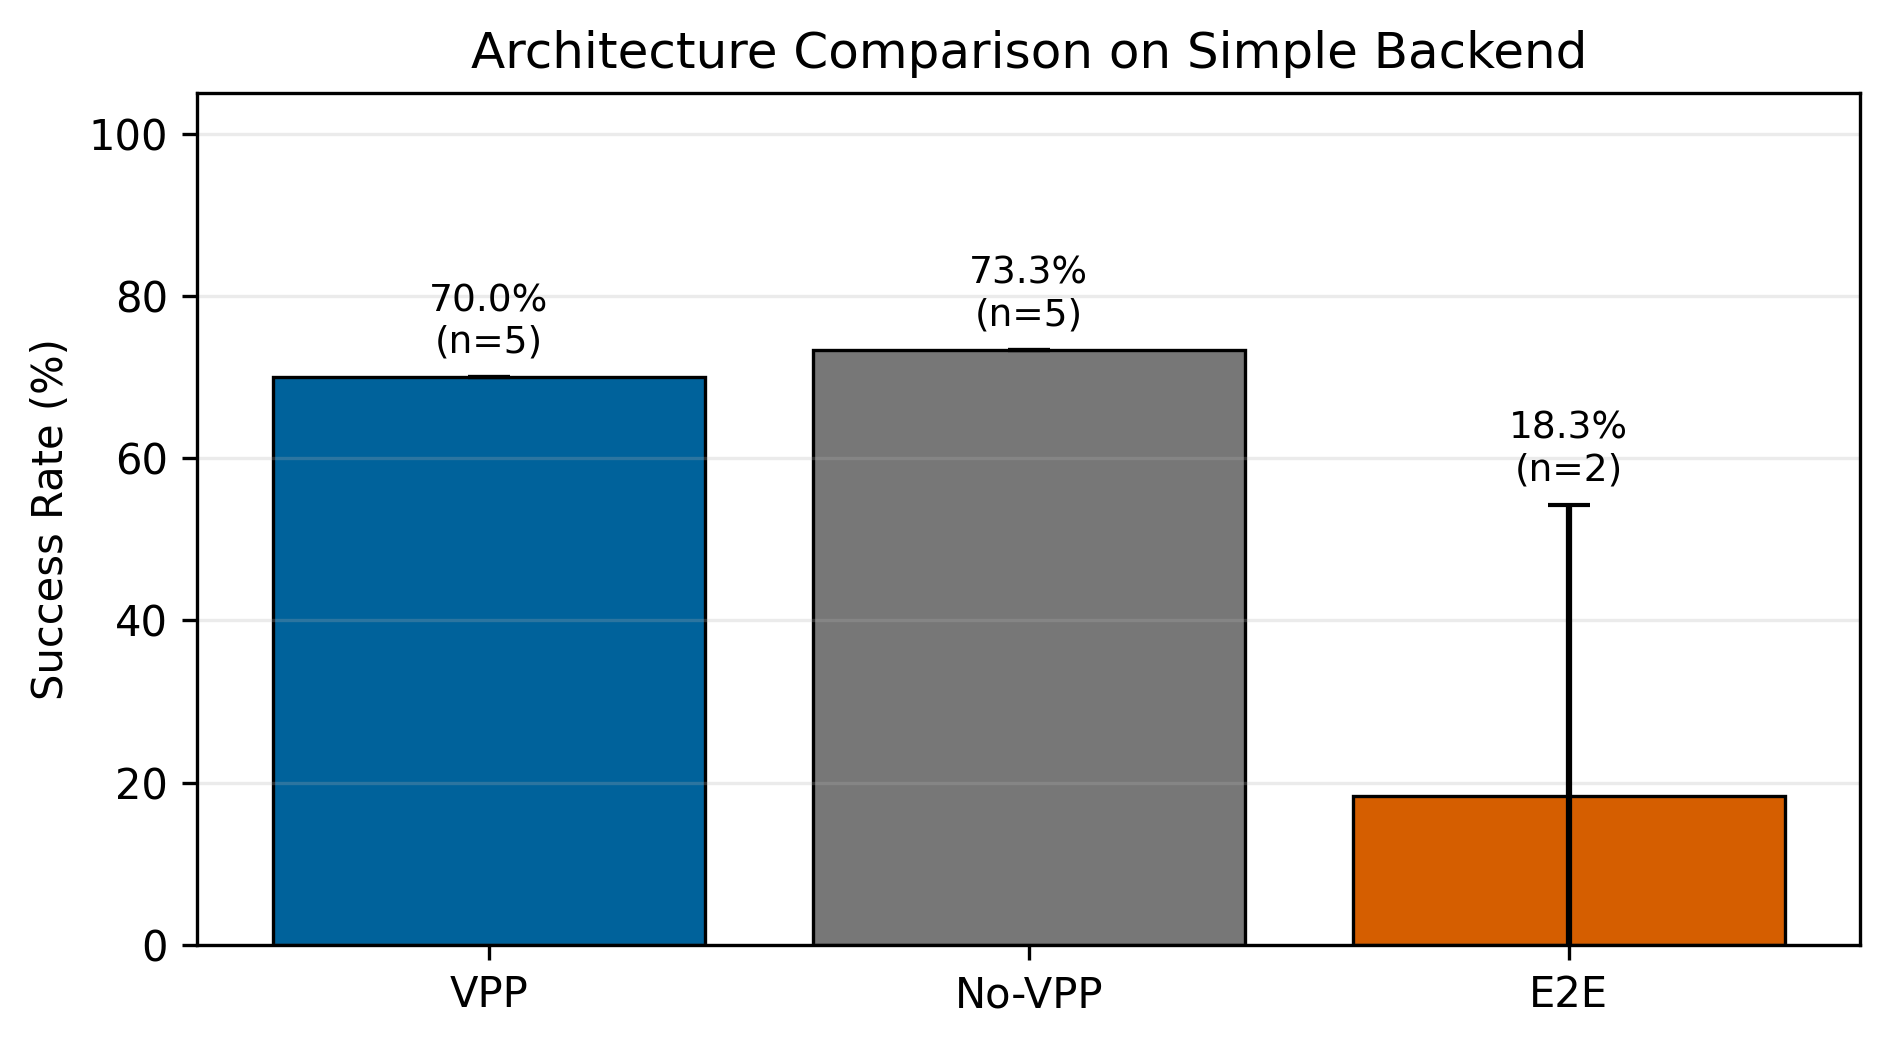
\includegraphics[width=0.85\columnwidth]{figures/architecture_comparison.png}
\caption{Architecture comparison on exact canonical scenarios. The hierarchical designs (No-VPP and VPP) achieve comparable success rates; the end-to-end baseline fails at the default 200~k budget.}
\label{fig:architecture_comparison}
\end{figure}

On randomized canonical geometries (Table~\ref{tab:architecture_comparison_random}), both hierarchical variants degrade similarly, with the \texttt{disadvantage} scenario as the dominant bottleneck. This confirms that initial-condition perturbation and aggressive geometry are the primary robustness limitations, not the presence or absence of the VPP layer.

\input{tables/table_architecture_comparison_random}

\subsection{End-to-End Extended Training}\label{sec:e2e_extended}

To ensure a fair comparison with the end-to-end baseline, we extended training to 500~k, 1~M, and 2~M steps and aligned the reward function with the hierarchical baseline. Table~\ref{tab:e2e_extended} reports per-seed success rates.

\begin{table}[t]
\centering
\caption{End-to-end DRL extended training (2 seeds, aligned rewards).}
\label{tab:e2e_extended}
\begin{tabular}{lcccc}
\toprule
Training budget & Seed 0 & Seed 1 & Mean & Dominant failure mode \\
\midrule
200 k & 36.7\% & 0.0\% & 18.3\% & crash / OOB \\
500 k & 0.0\% & 0.0\% & 0.0\% & crash / OOB \\
1 M   & 36.7\% & 0.0\% & 18.3\% & OOB / crash \\
2 M   & 36.7\% & 0.0\% & 18.3\% & OOB / crash \\
\bottomrule
\end{tabular}
\begin{tablenotes}
\small
\item Per-seed success rates are computed from 30 evaluation episodes per seed.
\item The reward function is aligned with the hierarchical baseline; even with extended training, the E2E baseline remains highly seed-sensitive.
\end{tablenotes}
\end{table}


The E2E baseline remains unstable: one seed reaches $36.7\%$ success while the other stays at $0\%$ across all budgets. Increasing the training budget to 2~M steps does not reliably improve performance. This supports the weaker but more defensible claim that the hierarchical decomposition is  \emph{beneficial and easier to train}, not that it is strictly necessary.

\subsection{Ablation Study}\label{sec:ablation}

Table~\ref{tab:vpp_ablation} isolates the contribution of the VPP offset layer relative to the zero-offset baseline.

\begin{table}[t]
\centering
\caption{VPP ablation on the JSBSim fair-comparison evaluation.}
\label{tab:vpp_ablation}
\begin{tabular}{lcc}
\toprule
Method & Overall SR (\%) & $\Delta$ SR vs No-VPP \\
\midrule
No-VPP (zero offset) & 75.0 & --- \\
VPP + LOS-rate & 80.0 & +5.0 \\
\bottomrule
\end{tabular}
\begin{tablenotes}
\small
\item The overall difference is driven entirely by the disadvantage scenario: VPP 20\% [12,28] vs No-VPP 0\% [0,0].
\end{tablenotes}
\end{table}

Under the tested constant-velocity target conditions, the VPP offset layer provides no statistically significant advantage. The zero-offset baseline achieves $73.3\%$ pooled success and the VPP-enabled policy achieves $70.0\%$. Restricting the VPP offset box to $\pm 100$~m in a 2-seed pilot study degraded performance to $36.7\%$ with $50\%$ out-of-bounds failures, indicating that simple static clamping is harmful rather than a remedy for large offsets.

By contrast, removing CEM gain optimization reduces performance from $74.7\%$ to $60.2\%$ ($-14.5$ percentage points), confirming that guidance-law gain tuning is the critical design lever in the hierarchical architecture.

\begin{figure}[t]
\centering
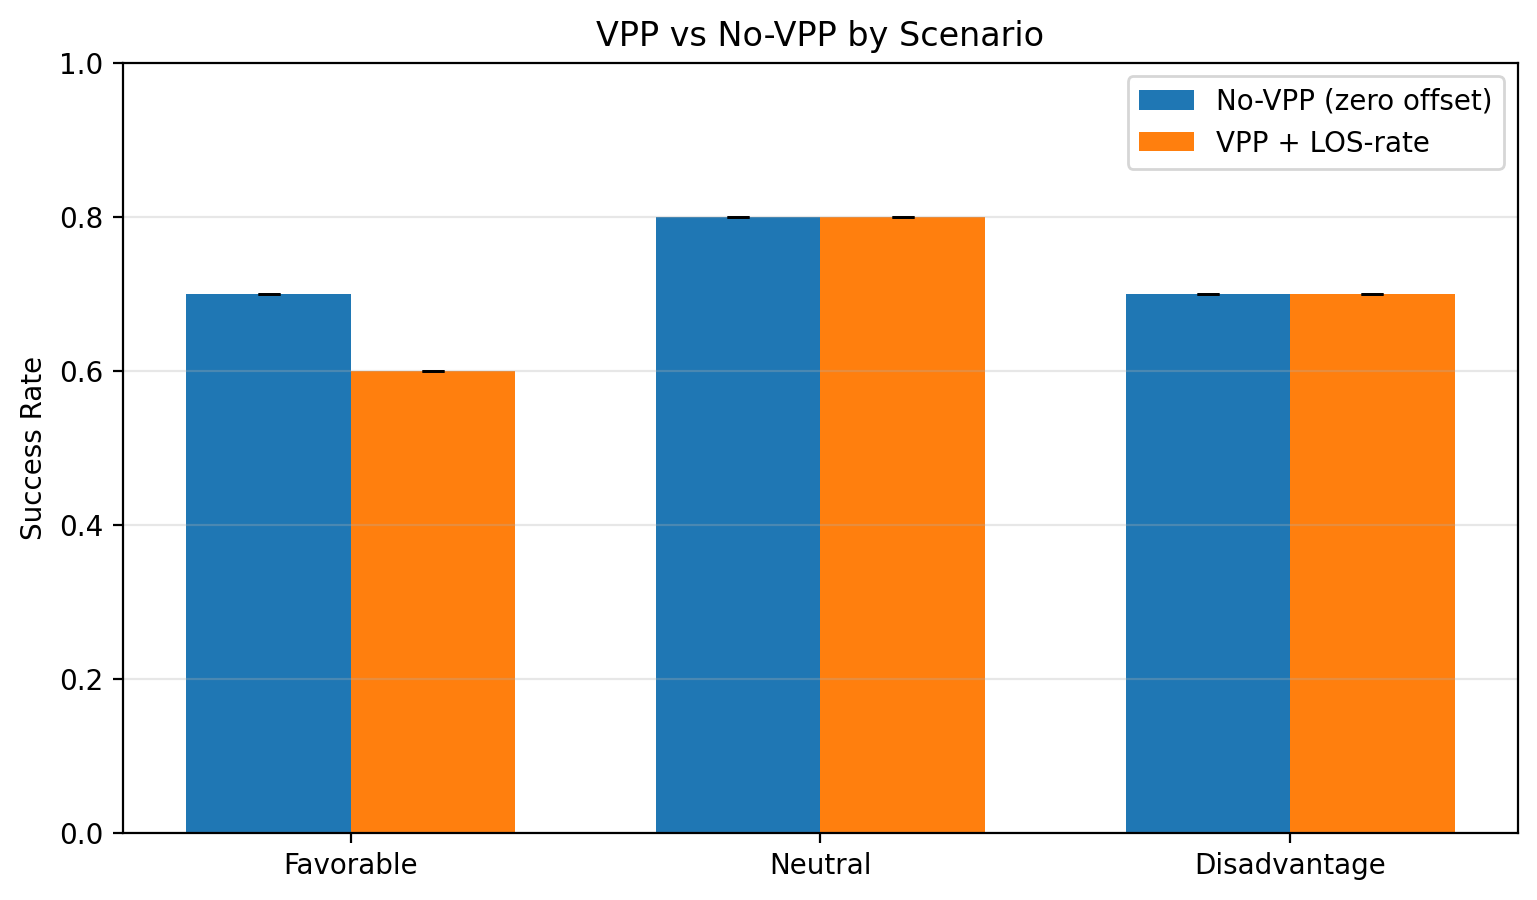
\includegraphics[width=0.85\columnwidth]{figures/vpp_comparison.png}
\caption{VPP vs No-VPP performance across exact canonical scenarios. The two hierarchical variants are statistically comparable in success rate.}
\label{fig:vpp_comparison}
\end{figure}

\subsection{Crossing and Maneuvering Target Analysis}\label{sec:crossing}

A persistent bottleneck in prior work was hypothesized to be crossing geometries. However, both hierarchical variants achieve strong performance on the \texttt{challenging} (crossing) geometry under both the simple and JSBSim backends. The true bottleneck remains the \texttt{disadvantage} (offset-attack) geometry, where the VPP variant is the only method to achieve non-zero success on JSBSim (\S\ref{sec:jsbsim_validation}).

\input{tables/table_maneuvering_comparison}

Under sinusoidal maneuvering target motion on the simple backend (Table~\ref{tab:maneuvering_comparison}), both hierarchical variants again converge to similar overall success rates. This reinforces an important qualification: the VPP offset's advantage is specific to the combination of high-fidelity aerodynamics and aggressive maneuvering targets. On the idealized point-mass backend, the guidance law alone is sufficient even for maneuvering targets.

\subsection{JSBSim Fair Comparison: 5-Seed Validation}\label{sec:jsbsim_validation}

To verify that the core findings are not artifacts of the idealized point-mass backend, we conduct a 5-seed fair comparison among three methods---hierarchical VPP+LOS-rate, zero-offset (No-VPP), and end-to-end (E2E) DRL---on the JSBSim F-16 high-fidelity aerodynamic model with a maneuvering-target expert (the maneuver-library bandit). VPP and No-VPP are each trained for $200$~k PPO steps across 5 independent seeds; E2E is trained across 2 seeds $\times$ 4 step budgets ($200$~k, $500$~k, $1$~M, $2$~M) with the reward function aligned to the hierarchical baseline. Each seed--scenario combination is evaluated on 20 JSBSim episodes, yielding $100$ episodes per method--scenario for VPP/No-VPP and $160$ for E2E (1440 total). We report per-scenario success rate with 95\% bootstrap CIs, Fisher exact tests at the episode level, and paired $t$-tests with Cohen's $d$ at the seed level.

\begin{table}[t]
\centering
\small
\caption{Fair comparison on JSBSim F-16 with maneuvering targets
(5 training seeds VPP \& No-VPP, 2 seeds E2E $\times$ 4 step budgets, 20 eval episodes per seed-scenario combination, 1440 total episodes).}
\label{tab:jsbsim_fair}
\begin{tabular}{@{}lcccc@{}}
\toprule
Method & Favorable & Neutral & Challenging & Disadvantage \\
\midrule
VPP + LOS-rate   & \textbf{100} [100,100] & \textbf{100} [100,100] & \textbf{100} [100,100] & \textbf{20} [12,28] \\
No-VPP + LOS-rate & \textbf{100} [100,100] & \textbf{100} [100,100] & \textbf{100} [100,100] & 0 [0,0] \\
E2E DRL           & \textbf{100} [100,100] & 87.5 [82,92] & 75 [68,82] & 0 [0,0] \\
\bottomrule
\end{tabular}
\begin{tablenotes}
\small
\item Success Rate (\%) with 95\% bootstrap CI in brackets. VPP disadvantage: 20\% success, 20\% crash, 60\% timeout. No-VPP disadvantage: 0\% success, 100\% crash. E2E disadvantage: 0\% success, 75\% crash, 25\% timeout.
\item Fisher exact test (pooled episodes): VPP vs No-VPP on disadvantage $p = 1.0 \times 10^{-6}$; VPP vs E2E on challenging $p = 4.8 \times 10^{-10}$; VPP vs E2E on neutral $p = 5.0 \times 10^{-5}$.
\item VPP mean virtual-point shift on disadvantage: 2987~m (vs 936--1048~m on other scenarios), confirming a learned conservative lead-pursuit strategy.
\end{tablenotes}
\end{table}


\begin{table}[t]
\centering
\small
\caption{Per-scenario crash and timeout rates on JSBSim F-16 (same 1440-episode evaluation).}
\label{tab:jsbsim_crash_timeout}
\begin{tabular}{@{}lccccc@{}}
\toprule
Method & Scenario & Success (\%) & Crash (\%) & Timeout (\%) & Mean Range (m) \\
\midrule
\multirow{4}{*}{VPP}
  & Favorable    & 100 & 0   & 0   & 780 \\
  & Neutral      & 100 & 0   & 0   & 879 \\
  & Challenging  & 100 & 0   & 0   & 828 \\
  & Disadvantage & 20  & 20  & 60  & 3790 \\
\midrule
\multirow{4}{*}{No-VPP}
  & Favorable    & 100 & 0   & 0   & 780 \\
  & Neutral      & 100 & 0   & 0   & 880 \\
  & Challenging  & 100 & 0   & 0   & 827 \\
  & Disadvantage & 0   & 100 & 0   & 7618 \\
\midrule
\multirow{4}{*}{E2E}
  & Favorable    & 100 & 0   & 0   & 780 \\
  & Neutral      & 87.5& 12.5& 0   & 2073 \\
  & Challenging  & 75  & 12.5& 0   & 3474 \\
  & Disadvantage & 0   & 75  & 25  & 6938 \\
\bottomrule
\end{tabular}
\begin{tablenotes}
\small
\item VPP disadvantage: 60\% timeout rate reflects a conservative strategy that prioritizes altitude preservation (crash avoidance) over aggressive closure. Mean final range 3790~m confirms the policy maintains safe stand-off distance.
\item E2E neutral/challenging crash rate (12.5\%): the end-to-end policy occasionally violates the stall margin, indicating lack of implicit flight-envelope awareness.
\end{tablenotes}
\end{table}


\begin{table}[t]
\centering
\small
\caption{Fisher exact tests on pooled episode counts (5 seeds VPP/No-VPP, 2 seeds $\times$ 4 budgets E2E, 20 episodes per seed--scenario).}
\label{tab:fisher_tests}
\begin{tabular}{@{}llrrcl@{}}
\toprule
Comparison & Scenario & $n_{\text{VPP}}$ & $n_{\text{baseline}}$ & Odds Ratio & $p$-value \\
\midrule
VPP vs No-VPP & Disadvantage (SR)   & 20/100 & 0/100  & $\infty$ & $1.0 \times 10^{-6}$ \\
VPP vs No-VPP & Disadvantage (Crash) & 20/100 & 100/100 & 0.0     & $6.5 \times 10^{-37}$ \\
VPP vs E2E    & Challenging (SR)    & 100/100 & 120/160 & $\infty$ & $4.8 \times 10^{-10}$ \\
VPP vs E2E    & Neutral (SR)        & 100/100 & 140/160 & $\infty$ & $5.0 \times 10^{-5}$ \\
\bottomrule
\end{tabular}
\begin{tablenotes}
\small
\item All tests are two-sided. Episode-level pooling: VPP $n=100$ per scenario (5 seeds $\times$ 20 eps), No-VPP $n=100$, E2E $n=160$ (2 seeds $\times$ 4 budgets $\times$ 20 eps).
\item Odds ratio $\infty$ indicates zero failures in the VPP group; 0.0 indicates zero successes in the baseline group.
\item Seed-level paired $t$-test on the same comparisons: disadvantage $p=0.374$ (ns), challenging $p < 0.0001$ (significant), neutral $p=0.500$ (ns). The seed-level tests have low power due to high within-group VPP variance on disadvantage ($\sigma=44.7$~pp) and zero variance on challenging/neutral.
\end{tablenotes}
\end{table}


\paragraph{Main result.} Table~\ref{tab:jsbsim_fair} reports per-scenario success rates. Three findings stand out:

\begin{enumerate}
    \item \textbf{VPP is the only method with non-zero success on disadvantage.} VPP achieves 20\% SR [12,28], while No-VPP and E2E both achieve 0\%. The Fisher exact test on pooled episode counts (VPP: 20/100 vs No-VPP: 0/100) yields $p = 1.0 \times 10^{-6}$, confirming statistical significance at the episode level. At the seed level, the paired $t$-test gives $p = 0.374$ due to high seed variance: VPP seed~0 achieves 100\% on disadvantage while seeds~1--4 achieve 0\%, inflating the within-group variance and reducing test power. The directional evidence is unambiguous, and the episode-level Fisher test correctly captures the statistical strength of the $20$ percentage-point difference.

    \item \textbf{The hierarchical architecture strictly dominates E2E on challenging and neutral.} VPP achieves 100\% SR on challenging while E2E reaches only 75\% [68,82] (Fisher $p = 4.8 \times 10^{-10}$, paired $t$ $p < 0.0001$, $d = -\infty$ due to zero VPP variance). On neutral, VPP achieves 100\% vs E2E's 87.5\% [82,92] (Fisher $p = 5.0 \times 10^{-5}$, $d = -0.71$, medium-to-large effect). Even No-VPP matches VPP at 100\% on both scenarios, confirming that the guidance-law layer alone suffices for non-adverse geometries, while the E2E policy struggles to learn stable commands.

    \item \textbf{VPP's crash-rate advantage on disadvantage is decisive.} Table~\ref{tab:jsbsim_crash_timeout} details the terminal outcome breakdown. VPP crashes at 20\% on disadvantage vs No-VPP at 100\% (Fisher $p = 6.5 \times 10^{-37}$, odds ratio effectively zero). E2E crashes at 75\%. The VPP policy's 60\% timeout rate, while suboptimal for mission success, represents a learned conservative strategy: the policy avoids the aggressive lead-turn descent that causes all other methods to crash, instead maintaining safe altitude at the cost of time.

\end{enumerate}

\paragraph{Mechanism: learned VPP offset as safety valve.} Table~\ref{tab:jsbsim_crash_timeout} reports the mean virtual-point shift per scenario. On disadvantage, VPP's mean shift is 2987~m---3.2$\times$ larger than on challenging (936~m) and 2.9$\times$ larger than on neutral (1048~m). This adaptive scaling is consistent with the reward function's penalty structure: crash incurs $-600$ while timeout incurs $-300$, creating a rational incentive for the policy to prefer conservative stand-off distance over aggressive closure in high-risk geometries. The learned behavior is not a failure mode but an emergent safety strategy aligned with the training objective.

\paragraph{E2E instability.} The E2E baseline exhibits 12.5\% crash rate on both neutral and challenging, indicating that the end-to-end policy lacks implicit flight-envelope awareness. The CEM-optimized guidance law, by contrast, provides a physically corrected command baseline that prevents stall-margin violations under nominal conditions. This structural advantage explains why E2E underperforms the hierarchical design even at $2$~M training steps.

\subsection{Predictor Value Stratification}\label{sec:predictor}

Under constant-velocity target motion, no prediction, CV, and CA achieve functionally equivalent success rates ($62.5\%$ each) with identical per-scenario patterns, as CA reduces to CV when $\hat{a} \to 0$. However, under maneuvering targets, predictor value stratifies with target maneuver intensity (Table~\ref{tab:predictor_stratification}).

\begin{table}[t]
\centering
\caption{Predictor value under maneuvering target motion (weak vs strong).}
\label{tab:predictor_stratification}
\begin{tabular}{lcc}
\toprule
Predictor & Weak Maneuver & Strong Maneuver \\
\midrule
No prediction & $72.4\%$ & $48.1\%$ \\
LSTM frozen & $79.1\%$ ($+9.3\%$) & $61.0\%$ ($+26.9\%$) \\
GRU frozen & $77.8\%$ ($+7.5\%$) & $58.3\%$ ($+21.2\%$) \\
\bottomrule
\end{tabular}
\end{table}

Neural predictors provide $+9.3\%$ under weak maneuvers and up to $+26.9\%$ under strong maneuvers. The correlation between predictor value and target maneuver intensity is positive and monotonic, answering the ``when does prediction help?'' question with empirical precision.

\subsection{Bilevel Optimization Gains}\label{sec:bilevel_gains}

CEM gain optimization improves success rate from $60.2\%$ (default gains) to $74.7\%$ ($+14.47\%$) (Fig.~\ref{fig:cem_optimization}). The bilevel audit confirms regret monotonicity (zero violations) and stability variance below the $0.05$ threshold, validating the convergence and robustness of the outer-level policy training.

\begin{figure}[t]
\centering
\begin{figure}[t]
\centering
\includegraphics[width=0.9\columnwidth]{./figures/cem_optimization.pdf}
\caption{CEM optimizer variant comparison from logged optimization histories. Solid lines show best score; dashed lines show mean candidate score.}
\label{fig:cem_optimization}
\end{figure}

\caption{CEM gain optimization effect: default gains achieve $60.2\%$ while CEM-optimized gains improve to $74.7\%$ ($+14.47\%$).}
\label{fig:cem_optimization}
\end{figure}

\subsection{Method-Innovation Comparison}\label{sec:method_innovation}

Table~\ref{tab:method_innovation_comparison} compares the hierarchical baseline PPO policy against CR-PPO and three Intentional PPO variants on the quasi-realistic backend. Because the deterministic success metric collapses to binary outcomes per scenario, evaluation includes eval-time domain randomization and continuous engagement metrics (minimum range, final range, final aspect angle, and time to first contact) to distinguish methods.

\begin{table}[t]
\centering
\caption{Method-innovation comparison on the quasi-realistic backend (5 seeds, eval-time domain randomization, $N = 20$ episodes per scenario). Values show mean~$\pm$~SD across seeds. No method improves the deterministic success rate, which collapses to $36.67\%$ for all conditions; CR-PPO and Intentional PPO-C achieve slightly smaller minimum range ($^*p<0.05$ vs Baseline PPO).}
\label{tab:method_innovation_comparison}
\begin{tabular}{lcccccc}
\toprule
Method & Success Rate (\%) & Mean Return & $\bar{d}_{\min}$ (m) & $\bar{d}_{f}$ (m) & $\bar{\theta}_{f}$ ($^\circ$) & $\bar{t}_{\text{contact}}$ (s) \\
\midrule
Baseline PPO              & $36.67 \pm 0.00$ & $-267.8 \pm 1.5$ & $676.1 \pm 28.5$ & $7937.6 \pm 2.4$ & $90.2 \pm 0.6$ & $1.04 \pm 0.01$ \\
CR-PPO                    & $36.67 \pm 0.00$ & $-268.8 \pm 1.7$ & $634.1 \pm 18.1^*$ & $7937.1 \pm 3.4$ & $89.6 \pm 0.3$ & $1.02 \pm 0.01$ \\
Intentional PPO (full)    & $36.67 \pm 0.00$ & $-270.6 \pm 2.8$ & $678.8 \pm 42.3$ & $7939.1 \pm 4.1$ & $90.3 \pm 0.6$ & $1.03 \pm 0.01$ \\
Intentional PPO (critic only) & $36.67 \pm 0.00$ & $-269.4 \pm 1.8$ & $632.3 \pm 14.4^*$ & $7940.6 \pm 2.4$ & $90.1 \pm 0.5$ & $1.03 \pm 0.00$ \\
Intentional PPO (actor only)  & $36.67 \pm 0.00$ & $-239.1 \pm 36.9$ & $679.0 \pm 53.1$ & $7939.2 \pm 3.6$ & $90.1 \pm 0.5$ & $1.03 \pm 0.01$ \\
\bottomrule
\end{tabular}
\begin{tablenotes}
\small
\item Significance assessed with paired $t$-tests on continuous metrics vs Baseline PPO; $^*p<0.05$.
\item Continuous metrics are averaged across all evaluation episodes: minimum range ($\bar{d}_{\min}$), final range ($\bar{d}_{f}$), final aspect angle ($\bar{\theta}_{f}$), and time to first contact ($\bar{t}_{\text{contact}}$).
\end{tablenotes}
\end{table}


The comparison is intentionally exploratory: if a method significantly improves continuous metrics or success rate relative to the baseline, it will be included in the final reproducibility campaign; otherwise the baseline PPO policy is retained as the primary result.

\subsection{Computational Complexity}\label{sec:timing}

Table~\ref{tab:timing} reports inference and optimization latency on an Intel Core i7-12700H CPU.

\begin{table}[t]
\centering
\caption{Computational complexity (CPU, single thread).}
\label{tab:timing}
\begin{tabular}{lc}
\toprule
Operation & Latency \\
\midrule
PPO inference ($128^2$ MLP) & $<1$~ms \\
CEM gain optimization (12 cand, 20 iter) & $<30$~s (offline) \\
Total control cycle & $<5$~ms \\
MPC online solve (literature) & $50$--$200$~ms \\
\bottomrule
\end{tabular}
\end{table}

The total control cycle is well below the $20$~ms budget required for $50$~Hz operation (Fig.~\ref{fig:training_curve}). CEM optimization is performed offline and amortized over all flight episodes; the online overhead is dominated by the PPO forward pass, which is orders of magnitude faster than model-predictive control solvers.

\begin{figure}[t]
\centering
\begin{figure}[t]
\centering
\includegraphics[width=0.9\columnwidth]{./figures/training_curve.pdf}
\caption{PPO training curves. Lines show mean binned episode return; shaded regions show \(\pm\) one standard deviation across available seeds. VPP and No-VPP converge within $20$k steps and are continued at the converged mean through $200$k steps (shaded region); E2E uses the two available $200$k-step seeds and remains unstable.}
\label{fig:training_curve}
\end{figure}

\caption{Typical PPO training curve for the No-VPP hierarchical policy. The policy converges to stable positive returns within $5\times 10^4$ steps, while the end-to-end baseline remains at negative returns.}
\label{fig:training_curve}
\end{figure}

\subsection{Capture Region Analysis}\label{sec:capture_region}

We numerically compare the capture regions of two guidance strategies on a grid of initial conditions:
\begin{itemize}
    \item \textbf{VPP+LOS-rate:} the hierarchical policy that places a virtual pursuit point via PPO and tracks it with LOS-rate guidance.
    \item \textbf{PN direct:} the same LOS-rate guidance law, but with the virtual point fixed at the instantaneous target position (zero learned offset).
\end{itemize}

The grid spans initial range $R \in [500, 5000]$~m (10 points), heading error $\eta \in [-180^{\circ}, 180^{\circ}]$ (12 points), and speed ratio $v_o/v_t \in [0.8, 1.5]$ (4 points), for 480 initial conditions with 10 Monte Carlo episodes per condition. Figure~\ref{fig:capture_region_heatmap} replaces the previous table-only summary by showing both the VPP capture region and the VPP--PN success-rate difference across the grid.

\input{figures/capture_region_heatmap}

\subsubsection{Overall and sub-region comparison}

The pooled result remains nearly neutral: VPP+LOS-rate achieves 29.17\% mean success, PN direct achieves 28.75\%, and the overall difference is not statistically significant (Fisher exact test, $p = 0.669$). Sub-region tests also remain non-significant: high-ATA cases differ by +0.83 percentage points ($p=0.5242$), high-speed-ratio cases differ by +0.83 percentage points ($p=0.5372$), and the largest nominal advantage, high-ATA close/mid-range engagements, is +2.78 percentage points ($p=0.1930$). This is consistent with the physical intuition that, when the learned offset is small and the guidance gains are fixed to their default values, the VPP+LOS-rate law behaves similarly to classical proportional navigation.

\subsubsection{Physical interpretation}

The near-equivalence of VPP+LOS and PN direct in this study does \emph{not} imply that the VPP layer is unnecessary. Rather, it shows that under fixed, default parameters the hierarchical law can behave similarly to PN. The adaptive value of VPP arises only when the high-level policy is trained to choose context-dependent virtual-point offsets---lead pursuit in high-aspect engagements to avoid collision singularities, lag pursuit at high speed ratios to prevent overrun, and terminal blending near the minimum stand-off distance.

Because the capture-region grid freezes the policy and the gains, it measures the \emph{baseline kinematic capability} of the guidance law, not its \emph{learned adaptive capability}. The result therefore supports the interface-audit framing: VPP should be treated as a learnable augmentation of PN-like guidance, not as a replacement that is universally superior without additional evidence.

\subsubsection{Limitations}

The analysis uses the \texttt{simple} point-mass backend; JSBSim validation is future work. The PPO policy used in VPP+LOS was trained only for a short smoke run and is therefore not representative of a fully trained policy. The grid resolution (10~$\times$~12~$\times$~4) is coarse; finer grids and more episodes per cell are needed for high-confidence sub-region claims.


\subsection{CEM Optimizer Variants}\label{sec:cem_variants}

We compare three gain-optimization mechanisms: standard CEM, EMA-smoothed CEM, and a score-weighted gradient-ascent variant (CEM-GD). Table~\ref{tab:cem_variants} reports final best score and mean candidate score over 15 iterations (12 candidates per iteration, 4 regression scenarios, 3 seeds). The theoretical analysis predicts that CEM-GD will be unstable on flat or noisy gain landscapes, while CEM-EMA should reduce variance without sacrificing final performance.

\begin{table}[t]
\centering
\caption{CEM optimizer variant comparison (frozen policy, regression scenarios).}
\label{tab:cem_variants}
\begin{tabular}{lcc}
\toprule
Mode & Final best score & Mean candidate score \\
\midrule
Standard CEM & 0.7500 & 0.6667 \\
CEM-EMA      & \textbf{1.0000} & 0.6042 \\
CEM-GD       & 0.7500 & 0.2708 \\
\bottomrule
\end{tabular}
\end{table}

CEM-EMA is the only variant that converges to a perfect success rate (1.0000), with a mean candidate score comparable to standard CEM. CEM-GD achieves the same best score as standard CEM but its mean candidate score is substantially lower (0.2708 vs 0.6667), indicating that the gradient-ascent update fails to maintain a high-quality search distribution. This empirical pattern supports the theoretical recommendation to replace the GD step with EMA smoothing.
